\documentclass[dvipdfmx, dvipsnames]{beamer}
\usepackage{tikz}
\usetikzlibrary{matrix,shapes, decorations.pathreplacing, backgrounds, positioning}

\begin{document}
\frame{
\begin{figure}
\begin{tabular}{ccc}
inner product of \Huge $($

\begin{tikzpicture}
\draw[thick,->,color=RoyalBlue] (0,0)--(0.71,0.71); 
  \draw[thick,->,color=RedOrange] (0,0)--(0.51,0.86);
\end{tikzpicture}
$)$
&
\Large $>$
&
inner product of \Huge $($
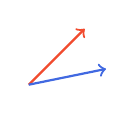
\begin{tikzpicture}
 \draw[thick,->,color=RedOrange] (0,0)--(0.71,0.71);
  \draw[thick,->,color=RoyalBlue] (0,0)--(0.98,0.2);
\end{tikzpicture}
$)$
\end{tabular}
\end{figure}
}
\end{document}

